\documentclass[]{beamer}

\mode<presentation>{\usetheme{default}\setbeamercovered{invisible}\usecolortheme{crane}}



\usepackage{natbib}
\bibliographystyle{abbrvnat}
\setcitestyle{authoryear,open={(},close={)}}

\usepackage{xcolor}
\usepackage{relsize}
\usepackage{listings}
\usepackage{verbatim}
\usetheme{Hannover}

\usepackage{varwidth}
\usepackage{xcolor}
\usepackage{lipsum}

\newcommand\MyCBox[1]{%
  \colorbox{red!60}{\begin{varwidth}{\dimexpr\linewidth-2\fboxsep}#1\end{varwidth}}}


\definecolor{LHCblue}{rgb}{0.29, 0.33, 0.13}
\usecolortheme[named=LHCblue]{structure}
\usepackage{textpos}
\usepackage{tikz}
\title{\textbf{\textcolor{blue}{Lab meeting 2015}}\\May 05}
\author{ }

\date{May 05, 2015}


\begin{document}
%%%%%%%%%%%%%%%%%%%%%%%%%%%%%%%%%%%%%%%%%%%%%%%%%%%%%%%%%%%%%%%%%%%%%%%%%%%%%%%%%%%%%%5
\section{Introduction}

%%%%%%%%%%%%%%%%%%%%%%%%%%%%%%%%%%%%%%%%%%%%%%%%%%%%%%%%%%%%%%%%%%%%%%%%%%%%%%%%%%%%%
\begin{frame}{}

\begin{itemize}
\item What is \LaTeX?
\item Why is it cool?
\end{itemize}

\end{frame}

%%%%%%%%%%%%%%%%%%%%%%%%%%%%%%%%%%%%%%%%%%%%%%%%%%%%%%%%%%%%%%%%%%%%%%%%%%%%%%%

%%%%%%%%%%%%%%%%%%%%%%%%%%%%%%%%%%%%%%%%%%%%%%%%%%%%%%%%%%%%%%%%%%%%%%%%%%%%%%%
\begin{frame}{What is \LaTeX?}

Google it:

\centering

\includegraphics[width = 7cm, height = 5cm]{WhatIsLatex.png}

\framebox{\bf{Myself: \LaTeX $\sim$ \bf{\textcolor{red}{Word}} $+$ \bf{\textcolor{red}{Power Point}}}}

\end{frame}
%%%%%%%%%%%%%%%%%%%%%%%%%%%%%%%%%%%%%%%%%%%%%%%%%%%%%%%%%%%%%%
\begin{frame}{Why is it cool?}

\centering
\bf{\textcolor{blue}{Please see what you can do with \LaTeX?}}

\vspace{1cm}
\centering

\includegraphics[with = 3cm, height = 3cm]{question-mark-face.jpg}

\end{frame}
%%%%%%%%%%%%%%%%%%%%%%%%%%%%%%%%%%%%%%%%%%%%%%%%%%%%%%%%%%%%%%%%%%
\section{\LaTeX}

\subsection{Equation}

\begin{frame}[fragile] \frametitle{No mouse to write any complex equations}


\includegraphics[width = 1.2cm, height = 1.2cm]{SmileFace.png}

\vspace{0.8cm}
Example \footnote{Source: http://en.wikibooks.org/wiki/LaTeX/Mathematics}:

\centering
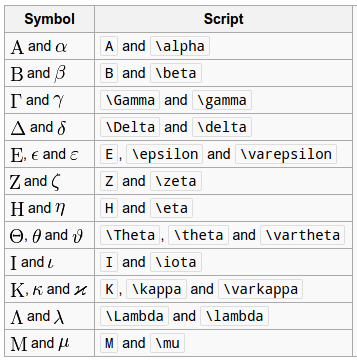
\includegraphics[width = 4.5cm, height = 4.5cm]{mathSource.png} & \\
\end{frame}

%%%%%%%%%%%%%%%%%%%%%%%%%%%%%%%%%%%%%%%%%%%%%%%%%%%%%%%%%%%%%%%%%%%%%%%%%%%%%%%%%%
\begin{frame}[fragile]


\textcolor{blue}{\bf{How can I write this sentence in \LaTeX?}}

\vspace{0.8cm}

\tiny

$scoreP_j^{R} = \sum\limit_{i = 1}^{M_{g}}\sum\limits_{k=1}^{N_{breaks}} w_k^{R}*f(x_k) $ is so easy to write in \LaTeX. Please don't use Word to write such an equation.

\large

\vspace{1cm}
\textcolor{blue}{\bf{Just type:}}
\vspace{0.8cm}
\tiny


\begin{verbatim}

scoreP_j^{R} = \sum\limit_{i = 1}^{M_{g}}\sum\limits_{k=1}^{N_{breaks}} w_k^{R}*f(x_k) is easy 

to write in LaTeX. Please don't use Word to write such an equation.

\end{verbatim}

\end{frame}
%%%%%%%%%%%%%%%%%%%%%%%%%%%%%%%%%%%%%%%%%%%%%%%%%%%%%%%%%%%%%%%%%%%%%%%%%%%%%%%%%
\subsection{Picture/Table}
%%%%%%%%%%%%%%%%%%%%%%%%%%%%%%%%%%%%%%%%%%%%%%%%%%%%%%%%%%%%%%%%%%%%%%%%%%%%%%%%
\begin{frame}[fragile]\frametitle{Adjust picture sizes}


Example: insert a picture named \underline{RStudioPicture.png}



\vspace{1cm}
\textcolor{blue}{\bf{SMALL? \\Just type}}

\tiny
\begin{verbatim}


\includegraphics[width = 1cm, height = 1cm]{RStudioPicture.png}

\end{verbatim}


\includegraphics[width = 2cm, height = 1cm]{RStudioPicture.png}

\end{frame}

%%%%%%%%%%%%%%%%%%%%%%%%%%%%%%%%%%%%%%%%%%%%%%%%%%%%%%%%%%%%%%%%%%%%%%%%%%%%%%%%%%
\begin{frame}[fragile]\frametitle{Adjust picture sizes}


Example: insert a picture named \underline{RStudioPicture.png}

\vspace{1cm}
\textcolor{blue}{\bf{LARGE? \\Just type}}

\tiny
\begin{verbatim}


\includegraphics[width = 3cm, height = 2.5cm]{RStudioPicture.png}

\end{verbatim}


\includegraphics[width = 3cm, height = 2.5cm]{RStudioPicture.png}

\end{frame}


%%%%%%%%%%%%%%%%%%%%%%%%%%%%%%%%%%%%%%%%%%%%%%%%%%%%%%%%%%%%%%%%%%%%%%%%%%%%%%%%%%
\begin{frame}[fragile]\frametitle{Adjust your table}

\vspace{-1cm}
\tiny
\bf{\textcolor{blue}{SMALL columns}

\begin{verbatim}
\begin{tabular}{|p{1cm}|p{1cm}|}
\hline
a & b\\
\hline
b & c\\
\hline
\end{tabular}
\end{verbatim}

\begin{tabular}{|p{1cm}|p{1cm}|}
\hline
a & b\\
\hline
b & c\\
\hline
\end{tabular}

\vspace{0.7cm}
\bf{\textcolor{blue}{LARGE and more columns, rows}

\tiny
\begin{verbatim}
\begin{tabular}{|p{2cm}|p{4cm}||p{2cm}|}
\hline
a & b & b1 \\
\hline
b & c & c1\\
\hline
d & d1 & 
\includegraphics[width = 0.3cm, height = 0.3cm]{SmileFace.png}  \\
\hline
\end{tabular}
\end{verbatim}

\begin{tabular}{|p{2cm}|p{4cm}||p{2cm}|}
\hline
a & b & b1 \\
\hline
b & c & c1\\
\hline
d & d1 & 
\includegraphics[width = 0.3cm, height = 0.3cm]{SmileFace.png} \\
\hline
\end{tabular}

\end{frame}

%%%%%%%%%%%%%%%%%%%%%%%%%%%%%%%%%%%%%%%%%%%%%%%%%%%%%%%%%%%%%%%%%%%%%%%%%%%%%%%%%
\subsection{Citation}
\begin{frame}[fragile]{Citation}

\tiny
\bf{\textcolor{blue}{Want to cite this paper?}

\includegraphics[width = 8cm, height = 2.1cm]{naturePaper.png}

\vspace{1cm}
\bf{\textcolor{blue}{Just type}}

\begin{verbatim}

\citet{chang2015core} published a cool paper. 

In 2015, \citeauthor{chang2015core} published a cool paper. 

\end{verbatim}

\bf{\textcolor{blue}{And see this}}

\citet{chang2015core} published a cool paper. 

In 2015, \citeauthor{chang2015core} published a cool paper. 

\vspace{1cm}
\tiny
\textit{*chang2015core} is a short name.

\end{frame}
%%%%%%%%%%%%%%%%%%%%%%%%%%%%%%%%%%%%%%%%%%%%%%%%%%%%%%%%%%%%%%%%%%%%%%%%%%%%%%%%%
\begin{frame}[fragile]{Citation: Natbib package}

\centering
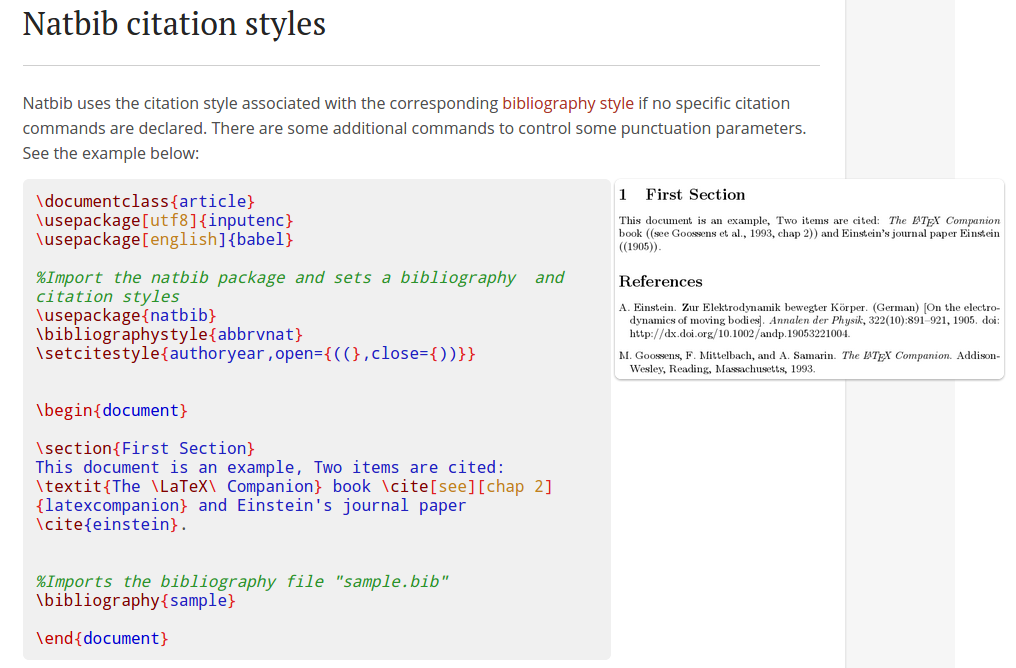
\includegraphics[width = 9cm, height = 8cm]{Natbib.png}

\end{frame}


%%%%%%%%%%%%%%%%%%%%%%%%%%%%%%%%%%%%%%%%%%%%%%%%%%%%%%%%%%%%%%%%%%%%%%%%%%%%%%%%%%%
\subsection{Thesis}
\begin{frame}[fragile]{Thesis}


\bf{\textcolor{blue}{Great!}} 

\vspace{0.7cm}

\tiny
\framebox{Don't want to spend time to adjust \textcolor{red}{tables + pictures + citations + formats ...}}

\vspace{0.7cm}
\large
\bf{\textcolor{blue}{$=>$ please just use \LaTeX.}}

\vspace{1cm}
Otago \LaTeX thesis package can be downloaded from:

\url{http://www.cs.otago.ac.nz/research/systems/resources.html}

\end{frame}
%%%%%%%%%%%%%%%%%%%%%%%%%%%%%%%%%%%%%%%%%%%%%%%%%%%%%%%%%%%%%%%%%%%%%%%%%%%%%%%%%
\subsection{Beamer}
\begin{frame}[fragile]{Presentation}



\centering
\bf{\textcolor{blue}{\LaTeX is used to make this presentation.}}

\vspace{1cm}
\centering
\bf{But how?}


\end{frame}
%%%%%%%%%%%%%%%%%%%%%%%%%%%%%%%%%%%%%%%%%%%%%%%%%%%%%%%%%%%%%%%%%%%%%%%%%%%
\begin{frame}[fragile]{Presentation}

\bf{The magician \textcolor{blue}{``The Beamer package''}: you can customize (or copy) different themes}

$=>$ I usually download a theme and adjust it.

\vspace{0.8cm}
\centering
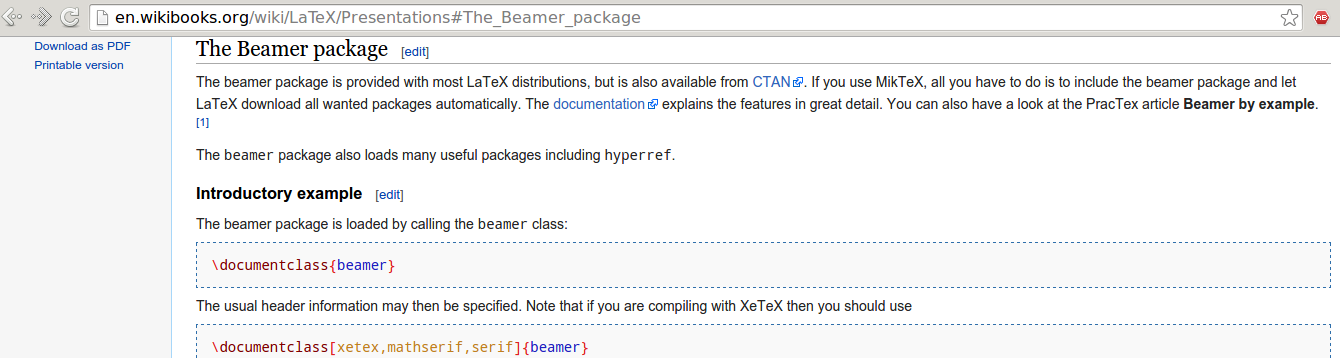
\includegraphics[width = 10cm, height = 4cm]{websiteBeamer.png}

\end{frame}
%%%%%%%%%%%%%%%%%%%%%%%%%%%%%%%%%%%%%%%%%%%%%%%%%%%%%%%%%%%%%%%%%%%%%%%%%%%%%%%%%
\begin{frame}{Beamer example}


\centering
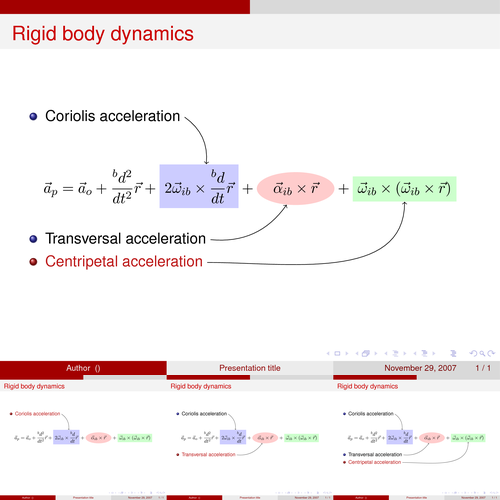
\includegraphics[width = 6cm, height = 6cm]{beamer1}
\end{frame}

%%%%%%%%%%%%%%%%%%%%%%%%%%%%%%%%%%%%%%%%%%%%%%%%%%%%%%%%%%%%%%%%%%%%%%%%%%%%%%%%5
\begin{frame}{Beamer example}


\centering
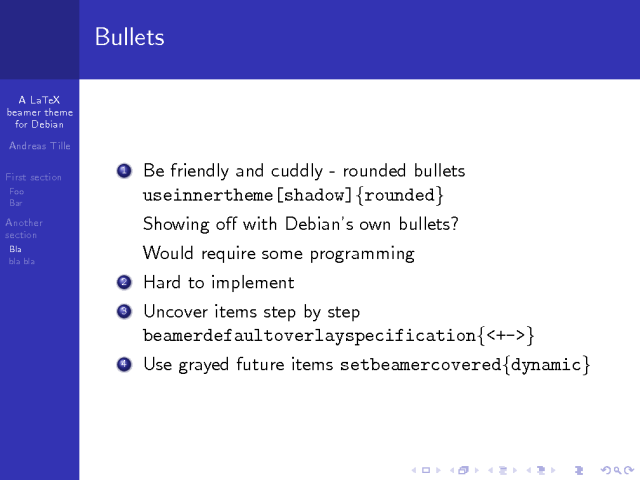
\includegraphics[width = 6cm, height = 6cm]{beamer2}

\end{frame}

%%%%%%%%%%%%%%%%%%%%%%%%%%%%%%%%%%%%%%%%%%%%%%%%%%%%%%%%%%%%%%%%%%%%%%%%%%%%%%%%%%%
\begin{frame}{Beamer example}


\centering

\includegraphics[width = 6cm, height = 6cm]{beamer3}

\end{frame}

%%%%%%%%%%%%%%%%%%%%%%%%%%%%%%%%%%%%%%%%%%%%%%%%%%%%%%%%%%%%%%%%%%%%%%%%%%%%%%%%%%%
\begin{frame}{Beamer example}


\centering
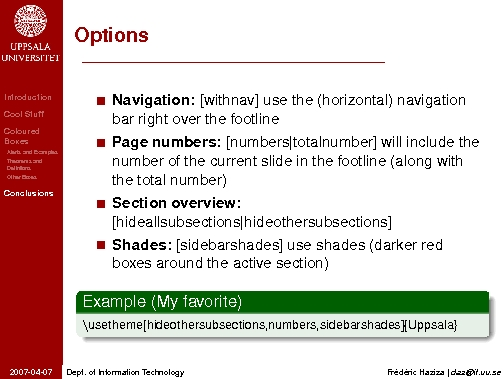
\includegraphics[width = 6cm, height = 6cm]{beamer4}

\end{frame}

%%%%%%%%%%%%%%%%%%%%%%%%%%%%%%%%%%%%%%%%%%%%%%%%%%%%%%%%%%%%%%%%%%%%%%%%%%%%%%%%%%%
\subsection{Example}
\begin{frame}{}
\vspace{-0.4cm}
Open emacs/vim/word...and type it, then go to terminal to compile it with \textit{pdflatex} and \textit{bibtex}.
\hspace{-0.5cm}
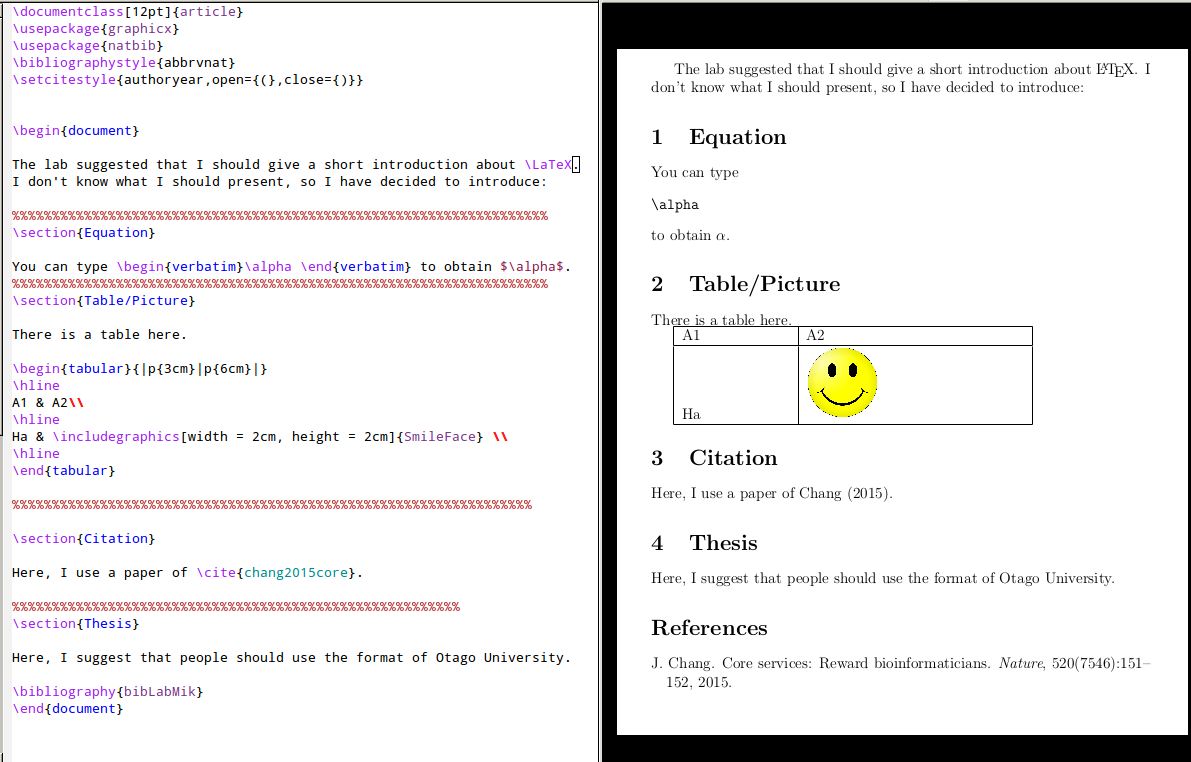
\includegraphics[width = 10.5cm, height = 8cm]{fullExample.png}

\end{frame}
%%%%%%%%%%%%%%%%%%%%%%%%%%%%%%%%%%%%%%%%%%%%%%%%%%%%%%%%%%%%%%%%%%%%%%%%%%%%%%%%%%%%%
\section{Discussion}
\begin{frame}{Discussion}

You can use \LaTeX to:
\begin{enumerate}
\item write your thesis/proposal/manual.
\item make your presentation.
\end{enumerate}

\vspace{1cm}
However, you have to work with biologists, so MUST use Word to write papers.

\end{frame}

%%%%%%%%%%%%%%%%%%%%%%%%%%%%%%%%%%%%%%%%%%%%%%%%%%%
\bibliography{bibLabMik}
\end{document}
